\documentclass[10pt, a4paper]{article}

\usepackage[utf8]{inputenc}
\usepackage[english]{babel}
\usepackage[T1]{fontenc}
\usepackage{charter}
\usepackage{amsmath}
\usepackage{amssymb}
\usepackage{hyperref}
\usepackage{graphicx}
\usepackage{enumitem}
\usepackage{url}
\usepackage{multirow}
\usepackage{array}
\usepackage{subcaption}
\usepackage{setspace}
\usepackage{booktabs}
\usepackage[nocompress]{cite}
\usepackage{geometry}
\geometry{top=1.3cm,bottom=1.3cm,left=1.6cm,right=1.5cm}
\usepackage{xcolor}
\usepackage{listings}

\pagestyle{plain}


\lstset{basicstyle=\ttfamily,
  showstringspaces=false,
  commentstyle=\color{red},
  keywordstyle=\color{blue},
  basicstyle=\footnotesize	
  %backgroundcolor=\xcolor{backcolour}
}


\begin{document}

\begin{center}

\textbf{Introduction to Computer Vision -- Homework 2} \\[0.1cm]

\textbf{RA192617 -- Edgar Rodolfo Quispe Condori} \\[0.1cm]
\textbf{RA192618 -- Darwin Ttito Concha} \\[0.1cm]

Institute of Computing, University of Campinas (UNICAMP) \\
Campinas-SP, Brazil, 13083-852 \\
\end{center}
%\section{Input data}

In this project we use three different videos, the technical details for each video are shown in table~\ref{table:input}.

Complete results of the experiments are \href{https://drive.google.com/open?id=0Bx_3lNzg57uuelRFc2JGWjR5ZkE}{available at: \textit{this link}}. Successful stabilization with keypoints matching will be download in the directory \textbf{myoutput} with make command.
\begin{table}[H]
\centering
\begin{tabular}{|l|c|c|l|}
\hline
\multicolumn{1}{|c|}{\textbf{Name}} & \textbf{Time(seconds)} & \textbf{Frames \#} & \multicolumn{1}{c|}{\textbf{Problem}} \\ \hline
p2-1-0.avi & 20 & 198 & Scale \\ \hline
p2-2-0.av & 26 & 260 & Translation and Rotation \\ \hline
p2-2-0.avi & 10 & 104 & Rotation \\ \hline
\end{tabular}
\caption{Technical detail of input videos.}
\label{table:input}
\end{table}

The original videos were recorded in 30fps but we considers 10fps to reduce the experiments execution time. The size of each frame is $640\times 480$ pixels.

\section{Keypoints Detector and Descriptor}

The algorithms that we implemented are based on the ORB to detect and SIFT to describe keypoints, it has slithly modification that were done based in experimental results and requested task.

\subsection{Keypoints Detector} 
We used ORB like interest point detector. The original approach uses FAST(Features from Accelerated Segment Test) to detect interests points and assings an orientation based in the intensity centroid. 

Originaly, FAST uses non-maximal suppression for removing adjacent corners and machine learning to improve the performance of the algorithm. In our implementation we do not use machine learning because the explanation is not clear. Our implementation and experiment consider three parameters : 
\begin{itemize}
	\item \textit{Threshold}: this parameter define if the sixteen neighbors point are lighter, darker or similar to reference point.
	\item \textit{N} : condition to determine if a point is a keypoint(at least N consecutive neighbors must be lighter or darker to reference point).
	\item \textit{Non-Maximum Suppression}: this parameter removes adjacent corners that are too close between them.
\end{itemize}

FAST does not produce a measure of cornerness (it has large responses along edges). As similar to the original implementation of ORB we employ a Harris corner measure to order and select $N$ keypoints. Another limitaton of FAST is that it does not produce orientation. To compensate this issue we use a approach similar to SIFT(ORB use moments of the patch around the keypoint). This technique take a window around of each keypoint and collect gradient directions and magnitudes. Then, a histogram is created for this and the amount that is added to the bin of the histogram is proportional to the magnitud of gradient at each points. Also, we used a gaussian weighting function, this function is multiplied by the magnitude. The farther away, the lesser the magnitude added.

Figure~\ref{fig:keypoints} shows results with different parameter settings.

\begin{figure}[h!]
\centering
\begin{subfigure}{0.5\textwidth}
  \centering
  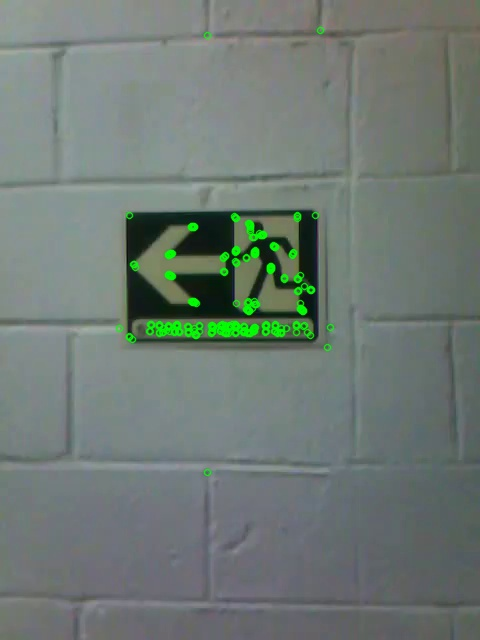
\includegraphics[width=0.5\linewidth]{figs/20-8-false-987.jpg}
  \caption{(20, 8, False). 987 keypoints detected}
\end{subfigure}%
\begin{subfigure}{0.5\textwidth}
  \centering
  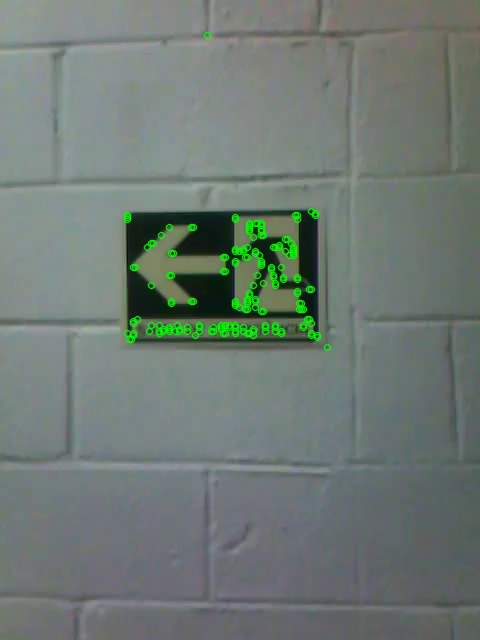
\includegraphics[width=0.5\linewidth]{figs/20-8-true-185.jpg}
  \caption{(20, 8, True). 185 keypoints detected}
\end{subfigure}
\begin{subfigure}{0.5\textwidth}
  \centering
  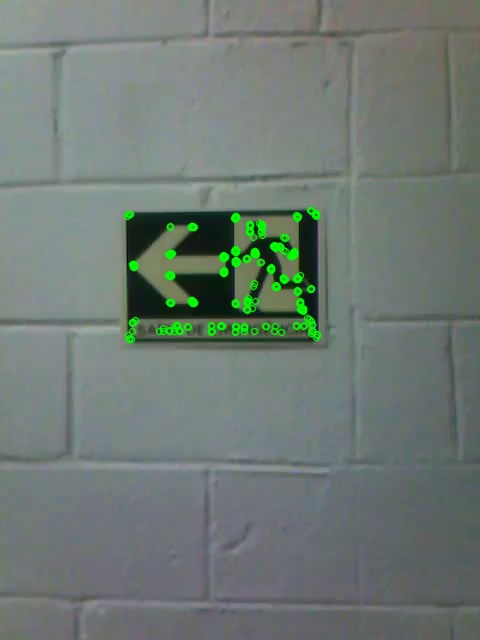
\includegraphics[width=0.5\linewidth]{figs/30-8-false-328.jpg}
  \caption{(30, 8, False). 328 keypoints detected}
\end{subfigure}%
\begin{subfigure}{0.5\textwidth}
  \centering
  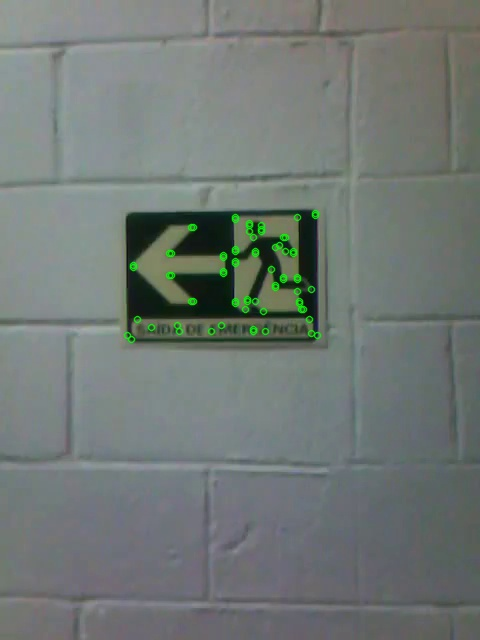
\includegraphics[width=0.5\linewidth]{figs/30-8-true-68.jpg}
  \caption{(30, 8, True). 68 keypoints detected}
\end{subfigure}
\begin{subfigure}{0.5\textwidth}
  \centering
  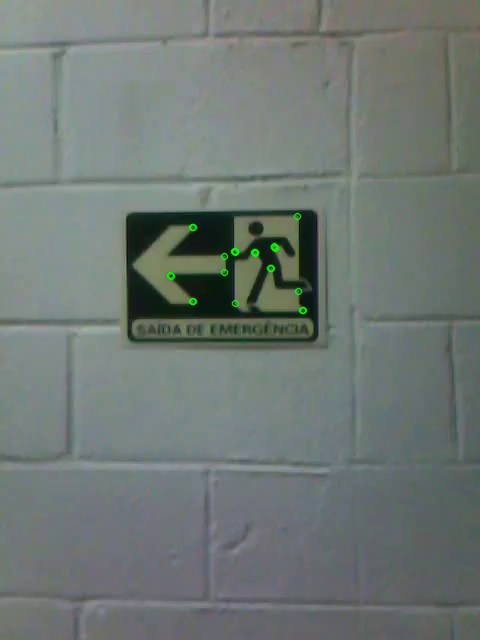
\includegraphics[width=0.5\linewidth]{figs/40-9-false-24.jpg}
  \caption{(40, 9, False). 24 keypoints detected}
\end{subfigure}%
\begin{subfigure}{0.5\textwidth}
  \centering
  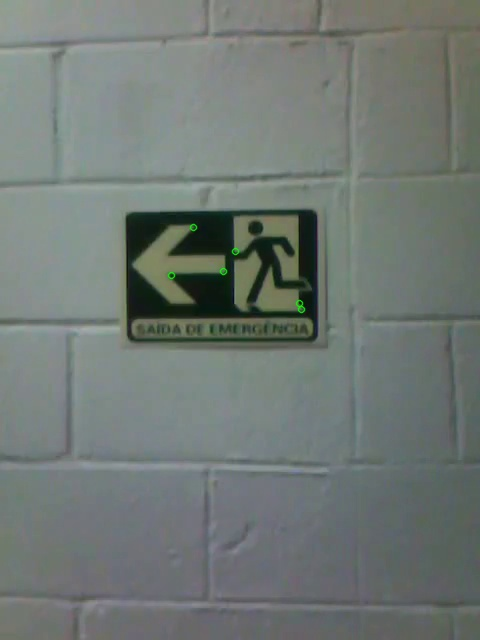
\includegraphics[width=0.5\linewidth]{figs/40-9-true-5.jpg}
  \caption{(40, 9, True). 6 keypoints detected}
\end{subfigure}
 \caption{Results of experiment with different parameter settings. The label of each subfigure follows the following format: \textit{(threshold, N, Non-maximum suppression)} and the number of keypoints detected.}
\label{fig:keypoints}
\end{figure}

Acording to figure~\ref{fig:keypoints} we can see that with parameter \textit{threshold}, the number of keypoints grows inversely proportional to its value. If we choose a too low value, we start getting falses positives and with a too big value, we start ignoring keypoints. This same effect occurs with the parameter $N$.

In the case of \textit{No-Maximal Suppresssion}, it removes close keypoints, but we have found that this redundancy of keypoints is util for stabilization.


\subsection{Keypoints Descriptor}

The original SIFT considers a pyramid in order to be invariant to scale, the keypoint descriptor is then computed from a specific level of this pyramid. Analysing the data it is easy to see that the scale differents between adjacent frame are negligibles. Thus, in our implementation ignores this stage in order to improve the performance of the algorithm.

Figure~\ref{fig:keypoints-match} shows results of the implementation.

\begin{figure}[h!]
\centering
\begin{subfigure}{0.5\textwidth}
  \centering
  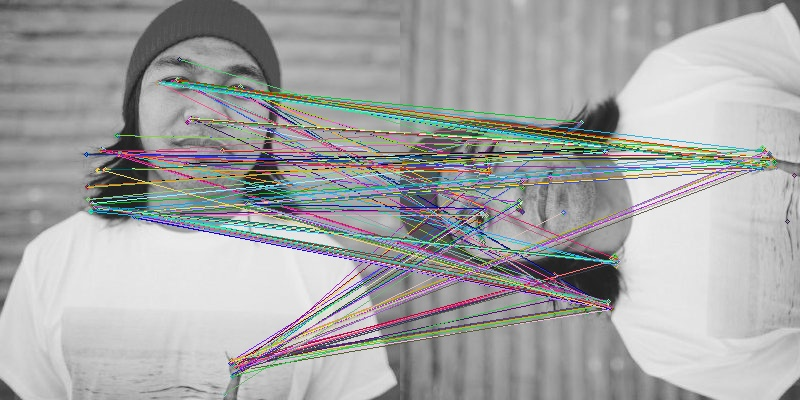
\includegraphics[width=0.9\linewidth]{figs/match-20-8-false.jpg}
  \caption{(20, 8, False).}
\end{subfigure}%
\begin{subfigure}{0.5\textwidth}
  \centering
  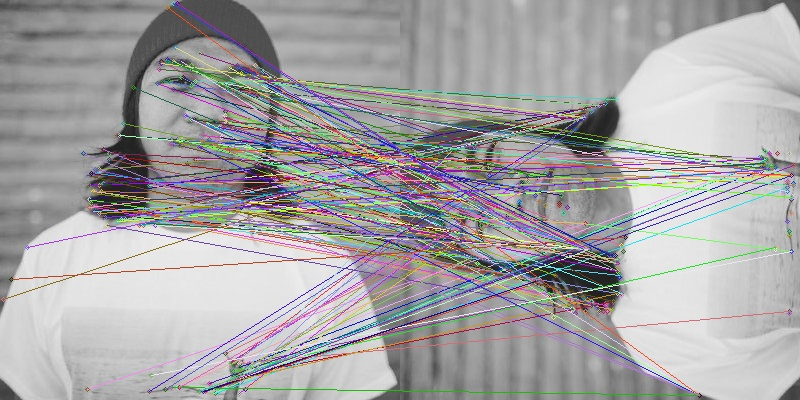
\includegraphics[width=0.9\linewidth]{figs/match-20-8-true.jpg}
  \caption{(20, 8, True).}
\end{subfigure}
\begin{subfigure}{0.5\textwidth}
  \centering
  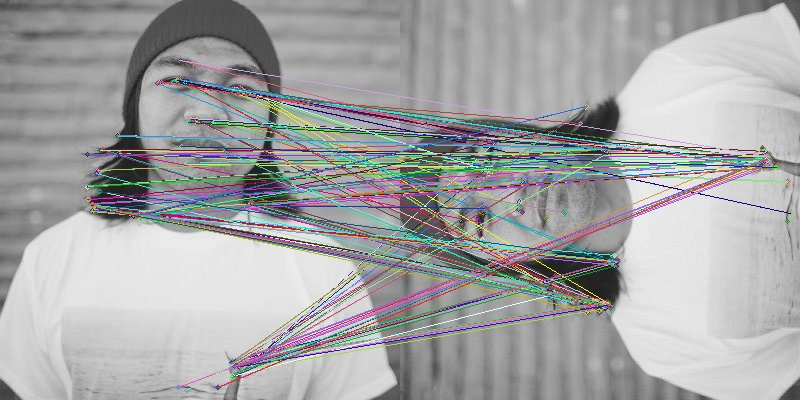
\includegraphics[width=0.9\linewidth]{figs/match-30-8-false.jpg}
  \caption{(30, 8, False).}
\end{subfigure}%
\begin{subfigure}{0.5\textwidth}
  \centering
  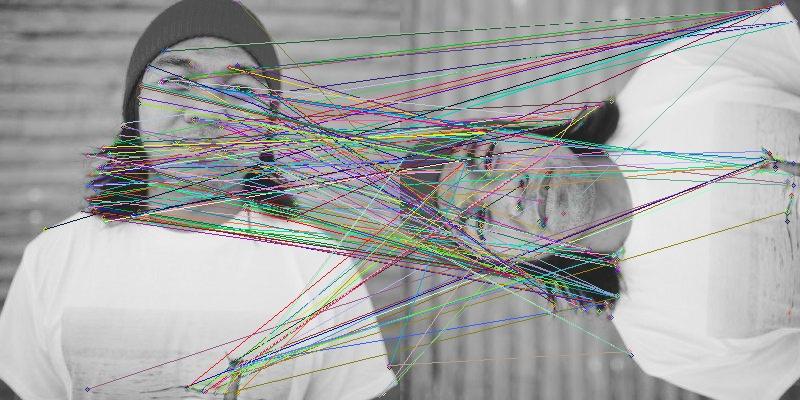
\includegraphics[width=0.9\linewidth]{figs/match-30-8-true.jpg}
  \caption{(30, 8, True).}
\end{subfigure}
\begin{subfigure}{0.5\textwidth}
  \centering
  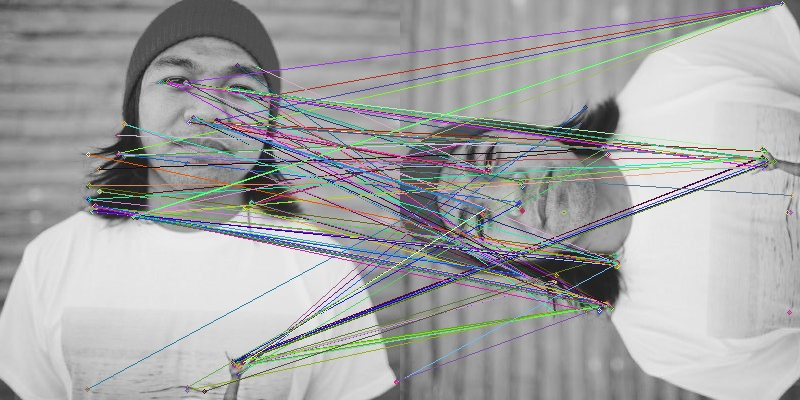
\includegraphics[width=0.9\linewidth]{figs/match-40-9-false.jpg}
  \caption{(40, 9, False).}
\end{subfigure}%
\begin{subfigure}{0.5\textwidth}
  \centering
  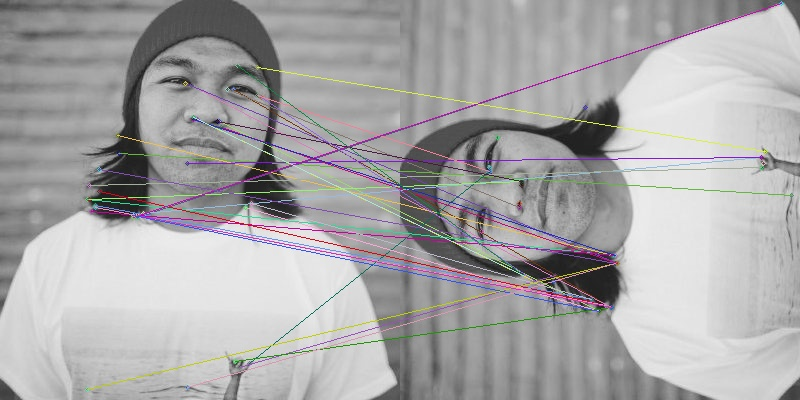
\includegraphics[width=0.9\linewidth]{figs/match-40-9-true.jpg}
  \caption{(40, 9, True).}
\end{subfigure}
 \caption{Results of matches with different parameter settings. The label of each subfigure follows the following format: \textit{(threshold, N, Non-maximum suppression)}}
\label{fig:keypoints-match}
\end{figure}

We can see in figure ~\ref{fig:keypoints-match} that the use of Non-Maximum Suppression create more outlier(wrong matches), this is because removing points that are close to one that will be correctly match decrease the number of inliers.


Our experiments suggest to use the setting of (30,8,False).  

\section{Match hypothesis}

Our implementation considers a simple match algorithm(brute force). For each keypoints of frame $i$ we find the closest match in the frame $i+1$ iterating over all possible candidates. We compare \textit{L2 Norm} and \textit{cosine} metrics to measure the similarity. Note that this implementation can generate the same match for two different keypoints yielding in an outlier.

An idea for performance improvement of this algorithm, is to use \textit{KNN(K-Nearest Neighbors)}. For real time application this may be a good option because its complexity is $O(n\log n)$, while our approach is $O(n^2)$ ($n$ is the number of keypoints).

Figure \ref{fig:diff-l2-cosine} shows the different result comparing \textit{L2 Norm} and \textit{cosine} metrics.


\begin{figure}[!h]
	\centering
	\begin{subfigure}{0.5\textwidth}
	  \centering
	  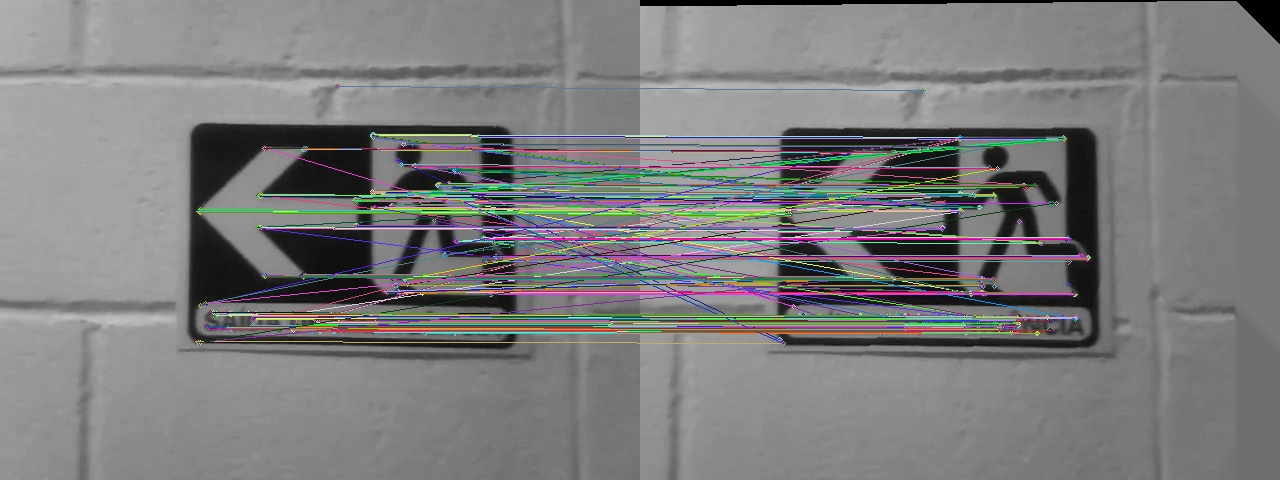
\includegraphics[width=0.9\linewidth]{figs/affine_100_cosine_30_8_False_p2-1-1_6-7.jpg}
	  \caption{Match hypothesis with cosine distance}
	\end{subfigure}%
	\begin{subfigure}{0.5\textwidth}
	  \centering
	  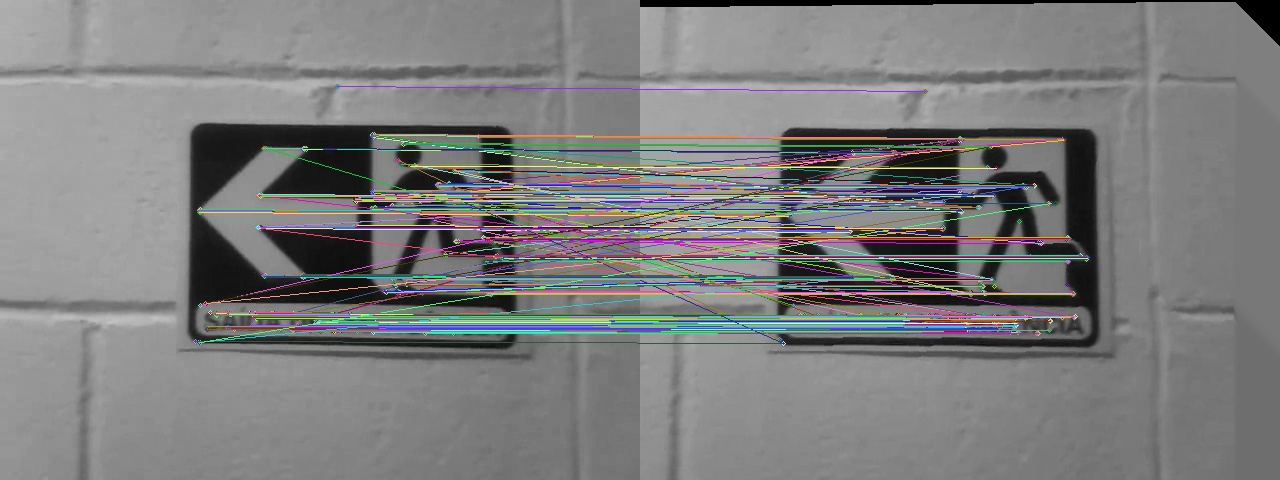
\includegraphics[width=0.9\linewidth]{figs/affine_200_l2-norm_30_8_False_p2-1-1_6-7.jpg}
	  \caption{Match hypothesis with l2-norm distance}
	\end{subfigure}
	\begin{subfigure}{0.5\textwidth}
        \centering
        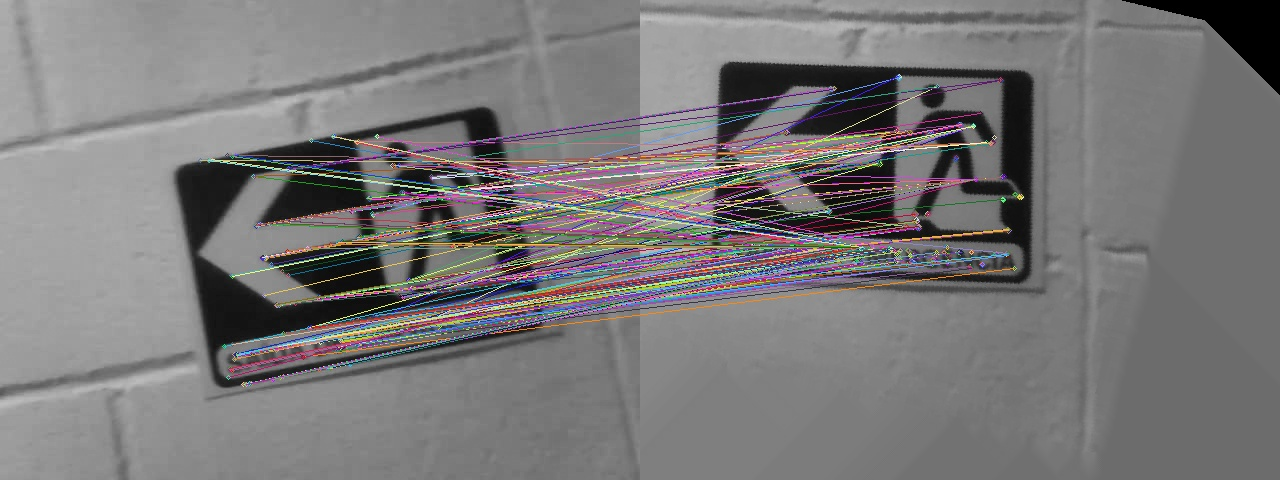
\includegraphics[width=0.9\linewidth]{figs/affine_100_cosine_30_8_False_p2-1-1_139-140.jpg}
        \caption{Match hypothesis with cosine distance}
      \end{subfigure}%
      \begin{subfigure}{0.5\textwidth}
        \centering
        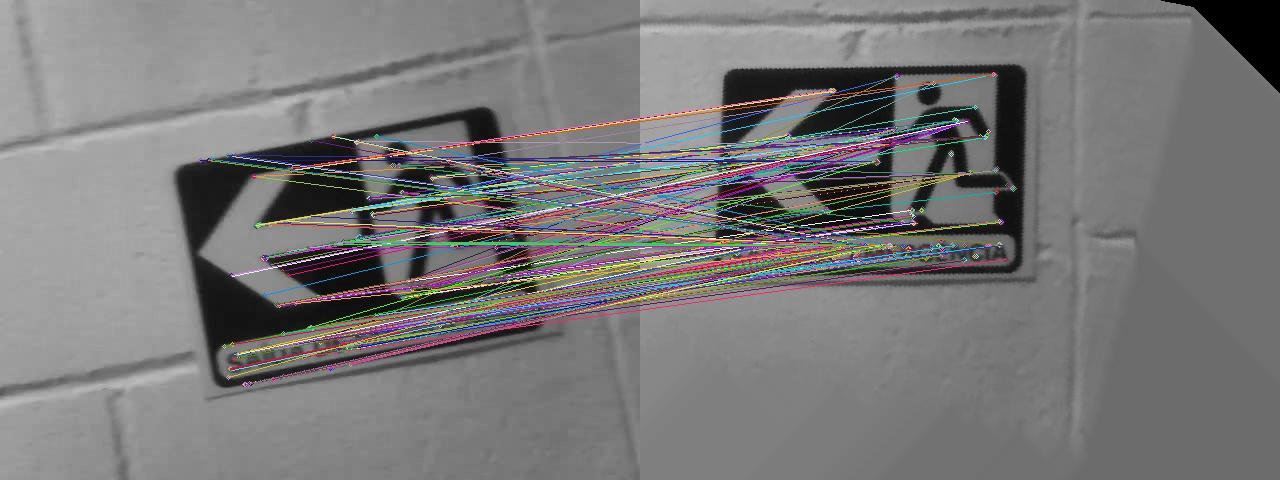
\includegraphics[width=0.9\linewidth]{figs/affine_200_l2-norm_30_8_False_p2-1-1_139-140.jpg}
        \caption{Match hypothesis with l2-norm distance}
      \end{subfigure}%
       \caption{Comparison of match hypothesis with cosine and l2-norm}
	\label{fig:diff-l2-cosine}
\end{figure}

We can see in figure ~\ref{fig:diff-l2-cosine} that the result of the experiment are very similar because there is not such an extreme difference between the performance of these metrics. There is an interesting difference in the execution time, as shown in table~\ref{table:dis-time}. L2-norm is slightly faster.  

\begin{table}[H]
\centering
\begin{tabular}{|l|c|c|}
\hline
\multicolumn{1}{|c|}{\multirow{2}{*}{\textbf{Name}}} & \multicolumn{2}{c|}{\textbf{Time per frame}} \\ \cline{2-3} 
\multicolumn{1}{|c|}{} & \textbf{L2-norm} & \textbf{Cosine} \\ \hline
p2-1-0.avi & 54.446 & 64.327 \\ \hline
p2-2-0.av & 37.321 & 42.982 \\ \hline
p2-2-0.avi & 54.446 & 45.262 \\ \hline
\end{tabular}
\caption{Execution time comparison.}
\label{table:dis-time}
\end{table}

We use \textit{cosine} distance as main similarity metric.

\section{Affine Tranformation Fitting}

Our implementation considers \textbf{Affine and Projective} tranformation.

The number of iteration of RANSAC has been determinated experimentaly, our implementation has the following modules:

\begin{lstlisting}[language=python][H]
def least_square(src, dst, matches, k_points, transformation = 'affine'):
def evaluate_transformation(src, dst, matches, trans_params, threshold = 1, evaluation_method = 'ramsac', transformation = 'affine'):
def ransac(src, dst, matches, k = 3, S = 35, threshold = 1, transformation = 'affine'):
\end{lstlisting}

\begin{itemize}
	\item \textit{least\_square}: this funtion creates the matrix $X,A$ and $Y$, depending of the parameter $transformation$. Given $N$ points $x_i, y_i (1\leq i\leq N ) $, in case of affine transformation, the matrix $X$ and $Y$ has to rows for each point:  
\[
X = 
\begin{bmatrix}
    x_{1}       & y_{1} & 1 & 0 & 0 & 0 \\
    0       & 0 & 0 & x_1 & y_1 & 1 \\
    x_{2}       & y_{2} & 1 & 0 & 0 & 0 \\
    0       & 0 & 0 & x_2 & y_2 & 1 \\
  \vdots & \vdots & \vdots & \vdots & \vdots & \vdots \\

    x_{N}       & y_{N} & 1 & 0 & 0 & 0 \\
    0       & 0 & 0 & x_N & y_N & 1 
\end{bmatrix}
%
Y = 
\begin{bmatrix}
    x'_{1} \\
    y'_{1} \\
    x'_{2}      \\
    y'_{2}   \\
 \vdots \\
    x'_{N}      \\
    y'_{N}   
\end{bmatrix}
\]

The parameters we want to find are defined for matrix $A$, in this case at least three points are needed and the transformation is computed using equation~\ref{eq:affine}.
\begin{equation}
\begin{split}
x'= ax+by+c \\
y'= dx+ey+f
\end{split}
\label{eq:affine}
\end{equation}

\[
A = 
\begin{bmatrix}
    a \\
    b \\
    c      \\
    d   \\ 
    e      \\
    f   
\end{bmatrix}
\]

In the case of the projective transformation, the matrix $X$ and $Y$ are defined by:

\[
X = 
\begin{bmatrix}
    x_{1}       & y_{1} & 1 & 0 & 0 & 0 & -x'_1x_1 & -x'_1y_1\\
    0       & 0 & 0 & x_1 & y_1 & 1 & -y'_1x_1 & -y'_1y_1\\
    x_{2}       & y_{2} & 1 & 0 & 0 & 0 & -x'_2x_2 & -x'_2y_2\\
    0       & 0 & 0 & x_2 & y_2 & 1 & -y'_2x_2 & -y'_2y_2 \\
  \vdots & \vdots & \vdots & \vdots & \vdots & \vdots \\

    x_{N}       & y_{N} & 1 & 0 & 0 & 0 & -x'_Nx_N & -x'_Ny_N\\
    0       & 0 & 0 & x_N & y_N & 1 & -y'_Nx_N & -y'_Ny_N 
\end{bmatrix}
%
Y = 
\begin{bmatrix}
    x'_{1} \\
    y'_{1} \\
    x'_{2}      \\
    y'_{2}   \\
 \vdots \\
    x'_{N}      \\
    y'_{N}   
\end{bmatrix}
\]
The parameters we want to find are defined for matrix $A$, in this case at least four points are needed and the transformation is computed using equation~\ref{eq:projective}.

\begin{equation}
\begin{split}
x'= ax+by+c-gx'x-hx'y\\
y'= dx+ey+f -gy'x-hy'y 
\end{split}
\label{eq:projective}
\end{equation}

\[
A = 
\begin{bmatrix}
    a \\
    b \\
    c      \\
    d   \\ 
    e      \\
    f   \\
    g\\
    h
\end{bmatrix}
\]

Matriz $A$ in both cases can be computed using least square. We use $numpy$ for easy implementation, sometimes the inverse does not exists, thus we return and empty vector.
\begin{lstlisting}[language=python][H]
x_transpose = np.matrix.transpose(X)
A = np.dot(x_transpose, X)
if np.linalg.det(A) == 0:
  print('Points', k_points, 'are not suitable for the transformation')
  return []
A = np.dot(np.linalg.inv(A), np.dot(x_transpose, Y))
return A
\end{lstlisting}

	\item \textit{evaluate\_transformation}: this function evaluates how many points fit correctly the compute transformation based on a threshold. The book suggests it to be between one and three. In our implementation we consider a value of two because our matches in the previous step are not perfect and we want to avoid missfitting because of outliers. The output of this function are the indexes of the points that fit the given parameters.

	\item \textit{ransac}: this function computes the RANSAC algorithm iterating $S$ times picking $k$ aleatory points. Our main assumptions is that least there is one valid solution that can be reached in $S$ iterations. The parameter $k$ is set to three for affine and four for proyective transformation.
\end{itemize}

\section{Transform}

In order to explain our algorithm consider the following notation: $i$ refers to the $i-th$ frame in the original video, and $i'$ refers to the $i-th$ frame in the stabilized video.

Initially, we considered the following algorithm to compute $i'$:
\begin{enumerate}
	\item extract keypoints($X$) from $(i-1)'$
	\item extract keypoints($Y$) from $i$
	\item find matches($M$) between $X$ and $Y$
	\item compute transformation $T$ from $M$.
	\item apply transformation $T$ to $i$
\end{enumerate}

With this approach, we were obtaining a lot of transformations errors(figure \ref{fig:misstransformations}) because the differences between $i$ and $(i-1)'$ are complex. Thus we defined anothe approach:   

\begin{figure}[!h]
	\centering
	\begin{subfigure}{0.5\textwidth}
	  \centering
	  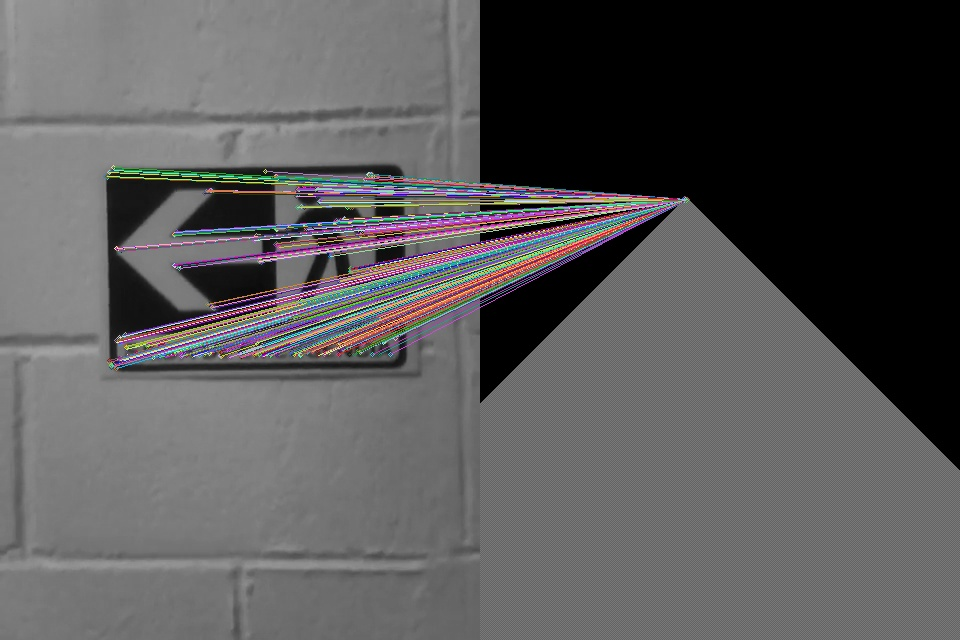
\includegraphics[width=0.8\linewidth]{figs/mistrans01.jpg}
	\end{subfigure}%
	\begin{subfigure}{0.5\textwidth}
	  \centering
	  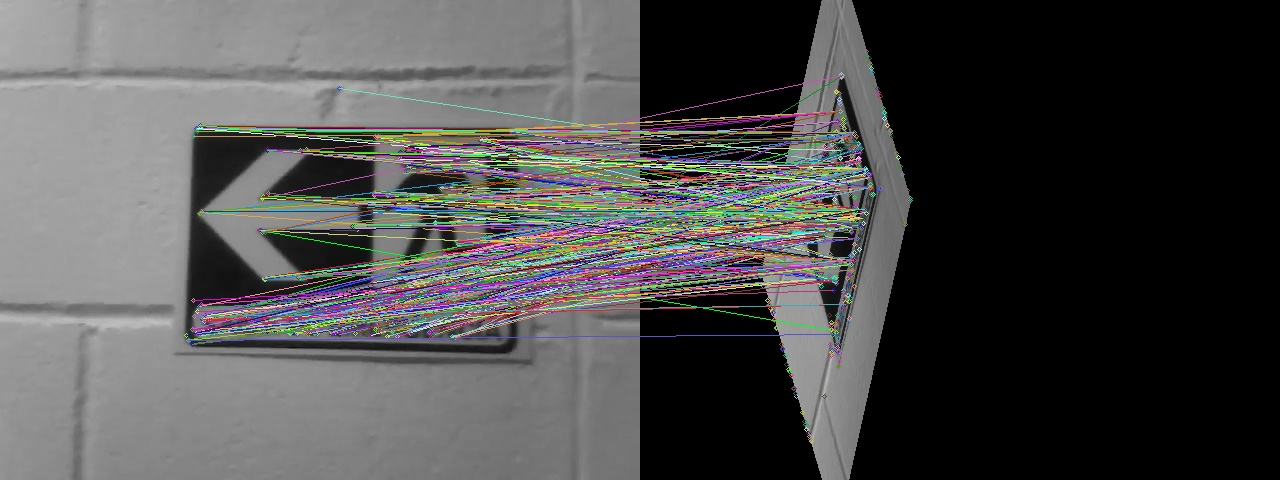
\includegraphics[width=0.8\linewidth]{figs/mistrans02.jpg}
	\end{subfigure}%
	 \caption{Errors of transformation using initial approach}
	\label{fig:misstransformations}
\end{figure}

\begin{enumerate}
	\item extract keypoints($X$) from $i-1$
	\item transform keypoints location of $i-1$ based on $(i-1)'$
	\item extract keypoints($Y$) from $i$
	\item find matches($M$) between $X$ and $Y$
	\item compute transformation $T$ from $M$.
	\item apply transformation $T$ to $i$
\end{enumerate}

We assume that the difference between adjacent frame in the original video is small. Thus, we compare the feature vector of $i$ and $i-1$, but the keypoints location of $i$ and $(i-1)'$.

Once we have the transformation of parameters we apply it for every pixel in $i$, depending of the movement, some black holes and lines appears(Figure \ref{fig:diff-interpolation}). Thus, we interpolate this points with the average of four neighbors and fill with zero the cases when the neighbors are also empty.

\begin{figure}[!h]
	\centering
	\begin{subfigure}{0.5\textwidth}
	  \centering
	  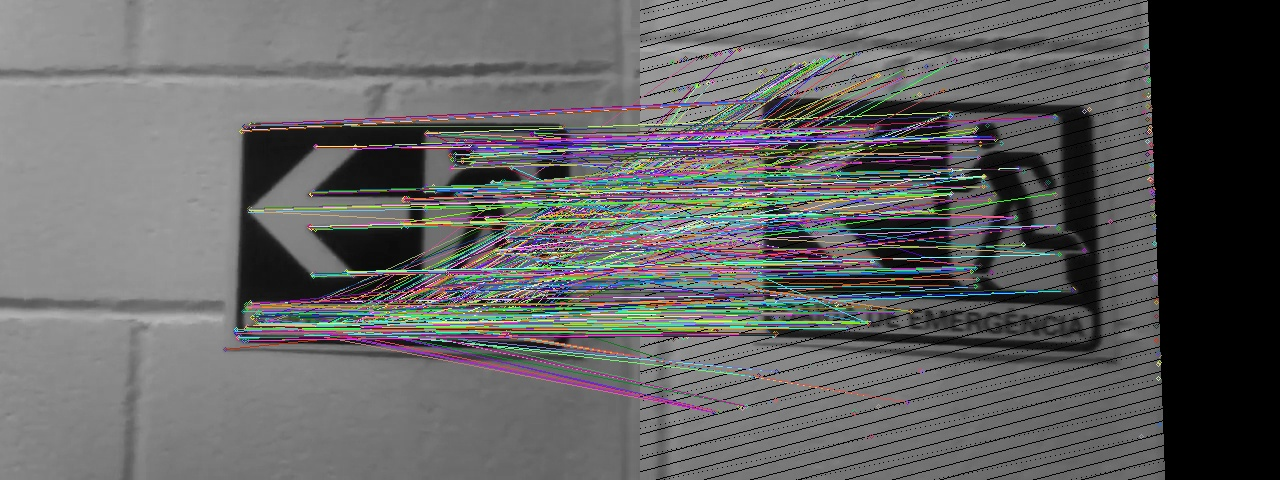
\includegraphics[width=0.8\linewidth]{figs/without-interpolation.jpg}
	  \caption{Without interpolation}
	\end{subfigure}%
	\begin{subfigure}{0.5\textwidth}
	  \centering
	  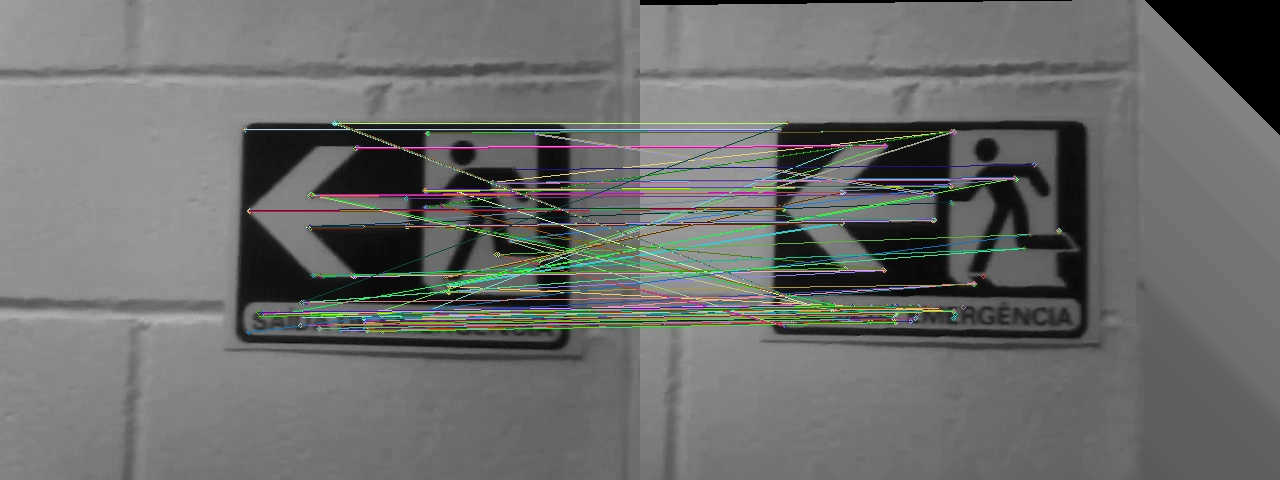
\includegraphics[width=0.8\linewidth]{figs/with-interpolation.jpg}
	  \caption{With interpolation}
	\end{subfigure}%
	 \caption{Comparison of results fof transformation uisng interpolation}
	\label{fig:diff-interpolation}
\end{figure}



result

L2-NORM
	VID0
	54.4464731615812
	24429436.7665
	VID1
	37.321051031466155
	29964112.0618
	VID2
	54.4464731615812
	24429436.7665

30-12 Orb
	VID0 fram 1
	43.35933494567871
	2330901497.0
	VID1 frame 11
	29.774162249131635
	89788339.9091
	VID2 frame 3
	22.77377374966939
	1185961909.67

NMS TRUE
	VID0 frame 37
	15.791857308811611
	42818733.9444
	VID1 frame 1
	16.9178147315979
	2531291808.0
	VID2 frame 14
	13.706815736634391
	194895992.714

S 200
	VID0
	62.691284131277634
	24540916.1218
	VID1
	42.43146139866597
	29430481.3977
	VID2
	45.6238714792196
	28768129.3107

S 100
	VID0
	64.32794978775954
	24672510.2183
	VID1
	42.98294043633008
	30052053.0116
	VID2
	45.26221292227217
	44096547.9223


S 36
	VID0
	62.32433629156974
	25921522.7817
	VID1 frame 205
	43.00332358523113
	44613346.3756
	VID2 frame 14
	46.593267457825796
	135858245.357

%\input{p2-3-2}

\end{document}
